\begin{table}[CU1 Tutor Socrático 1]{TB:CU1 1}{Caso de uso: Interacción con el tutor socrático. 1}
  \begin{tabular}{l p{11cm}}
    \hline
    \textbf{Campo} & \textbf{Descripción} \\
    \hline \hline
    \textbf{Identificador} & CU1 \\
    \textbf{Nombre} & Interacción con el tutor socrático \\
    \textbf{Actor principal} & Alumno (usuario autenticado) \\
    \textbf{Actores secundarios} & Ollama (LLM tutor), Ollama (LLM moderación) \\
    \textbf{Descripción} & El alumno envía una pregunta al tutor socrático, opcionalmente acompañada del código de su editor y la última salida de ejecución. El sistema modera la entrada, genera una respuesta pedagógica en streaming (SSE) y opcionalmente modera la salida en paralelo. \\
    \textbf{Precondiciones} & 1. El alumno está autenticado (posee un \texttt{access\_token} JWT válido). \newline  2. El servicio Ollama está activo y el modelo LLM configurado en \texttt{SystemConfig} está disponible. \newline  3. Existe una sesión de chat activa o se creará una nueva automáticamente. \\
    \textbf{Postcondiciones} & 1. El mensaje del alumno queda persistido en la tabla \texttt{Message} con \texttt{role='user'}. \newline  2. La respuesta del tutor queda persistida con \texttt{role='assistant'}. \newline  3. Si fue el primer mensaje, la sesión se renombra automáticamente (auto-naming). \newline  4. El campo \texttt{updated\_at} de la sesión se actualiza. \\
    \hline
  \end{tabular}
\end{table}

\begin{table}[CU1 Tutor Socrático 2]{TB:CU1 2}{Caso de uso: Interacción con el tutor socrático. 2}
  \begin{tabular}{c c p{8cm}}
    \hline
    \textbf{Paso} & \textbf{Actor} & \textbf{Acción} \\
    \hline \hline
    1 & Alumno & Escribe un mensaje en el chat y pulsa enviar. El frontend envía \texttt{POST /api/chat/} con \texttt{\{ session\_id, prompt, code\_context, last\_output, language \}}. \\
    2 & Sistema & Valida los datos de entrada mediante \texttt{ChatInputSerializer} (prompt $\le$ 2000 caracteres). \\
    3 & Sistema & Obtiene o crea la sesión de chat (\texttt{\_get\_or\_create\_session}). Si \texttt{session\_id} es \texttt{null}, crea una nueva sesión. \\
    4 & Sistema & Persiste el mensaje del alumno en la base de datos (\texttt{Message.objects.create}, \texttt{role='user'}). \\
    5 & Sistema & Ejecuta \texttt{\_auto\_name\_and\_touch}: si es el primer mensaje de usuario y el título es \texttt{''Nueva conversación''}, asigna los primeros 50 caracteres como título. Actualiza \texttt{updated\_at}. \\
    6 & Sistema & Lee la configuración global (\texttt{SystemConfig.get()}) para determinar: \texttt{llm\_model}, \texttt{moderation\_model} y \texttt{moderation\_mode}. \\
    7 & Sistema & \textbf{Moderación de input} (si \texttt{moderation\_mode $\in$ \{both, input\}}): invoca a \texttt{moderate\_input()} que envía el texto del alumno al LLM de moderación. El veredicto es \texttt{OK} $\rightarrow$ continúa. \\
    8 & Sistema & Construye el array de mensajes para Ollama: \texttt{SYSTEM\_PROMPT} + contexto de código (si existe) + últimos 10 mensajes del historial. \\
    9 & Sistema & Inicia el streaming asíncrono: \texttt{ollama.AsyncClient().chat(model=llm\_model, stream=True)}. Abre una respuesta \texttt{StreamingHttpResponse} con \texttt{content\_type='text/event-stream'}. \\
    10 & Sistema & Por cada token recibido, emite \texttt{data: \{''token'': ''...''\}} al frontend vía SSE. \\
    11 & Sistema & \textbf{Moderación de output} (si \texttt{moderation\_mode $\in$ \{both, output\}}): cada \texttt{MOD\_WORD\_WINDOW} palabras (20 por defecto), lanza un \texttt{asyncio.Task} que evalúa el texto acumulado hasta el momento. \\
    12 & Frontend & El \texttt{ReadableStream} del navegador procesa cada línea SSE. El callback \texttt{onToken(token)} concatena el token al mensaje del asistente en la interfaz de usuario, creando el efecto de escritura progresiva. \\
    13 & Sistema & Al finalizar el stream, emite \texttt{data: \{''session\_id'': N, ''session\_title'': ''...''\}} y \texttt{data: [DONE]}. Persiste la respuesta completa como \texttt{Message(role='assistant')}. \\
    14 & Frontend & El callback \texttt{onDone(sessionId, sessionTitle)} actualiza el estado de la sesión activa y el sidebar. \\
    \hline
  \end{tabular}
\end{table}

\begin{table}[CU1 Tutor Socrático 3]{TB:CU1 3}{Caso de uso: Interacción con el tutor socrático. 3}
  \begin{tabular}{c p{8cm} p{8cm}}
    \hline
    \textbf{ID} & \textbf{Condición} & \textbf{Acción del sistema} \\
    \hline \hline
    FA-01 & Moderación de input rechaza el mensaje (\texttt{NO}) & Se marca el mensaje del usuario como \texttt{moderated=True}. Se envía un stream con la respuesta predeterminada: \texttt{''Lo siento, no puedo procesar ese mensaje. ¿Puedes reformular tu pregunta?''} seguido de \texttt{[DONE]}. No se invoca al LLM tutor. \\
    FA-02 & Moderación de input falla por error técnico & Se aplica \textit{fail-closed}: el mensaje se trata como rechazado (se bloquea). Se devuelve la respuesta moderada predeterminada. \\
    FA-03 & Moderación de output rechaza un fragmento (\texttt{NO}) & Se interrumpe la generación del LLM (\texttt{break} en el bucle de streaming). Se emite \texttt{data: \{''moderated'': true, ''response'': ''...''\}} seguido de \texttt{[DONE]}. Se persiste el mensaje con \texttt{moderated=True} y el contenido de la respuesta predeterminada. \\
    FA-04 & Moderación de output falla por error técnico & Se aplica \textit{fail-open}: se permite continuar el stream sin interrupciones (\texttt{return True}). \\
    FA-05 & Error en el LLM durante el streaming & Se emite \texttt{data: \{''error'': ''Error en motor IA: <detalle>''\}} al frontend. El callback \texttt{onError(error)} muestra el error al usuario. \\
    FA-06 & Sesión no encontrada (\texttt{session\_id} inválido) & Se devuelve HTTP 404 con \texttt{\{''error'': ''Sesión no encontrada.'', ''details'': null\}}. \\
    FA-07 & Token JWT expirado o ausente & El frontend intercepta HTTP 401, intenta renovar el token automáticamente (\texttt{POST /api/auth/jwt/refresh/}). Si falla, redirige al login. \\
    FA-08 & Validación de entrada falla & Se devuelve HTTP 400 con los errores de validación en formato estandarizado \texttt{\{''error'': ''...'', ''details'': \{...\}\}}. \\
    \hline
  \end{tabular}
\end{table}

\begin{figure}[Diagrama de secuencia CU1]{FIG:CU1_SEQ}{Diagrama de secuencia de la interacción del chat con streaming.}
    \centering
    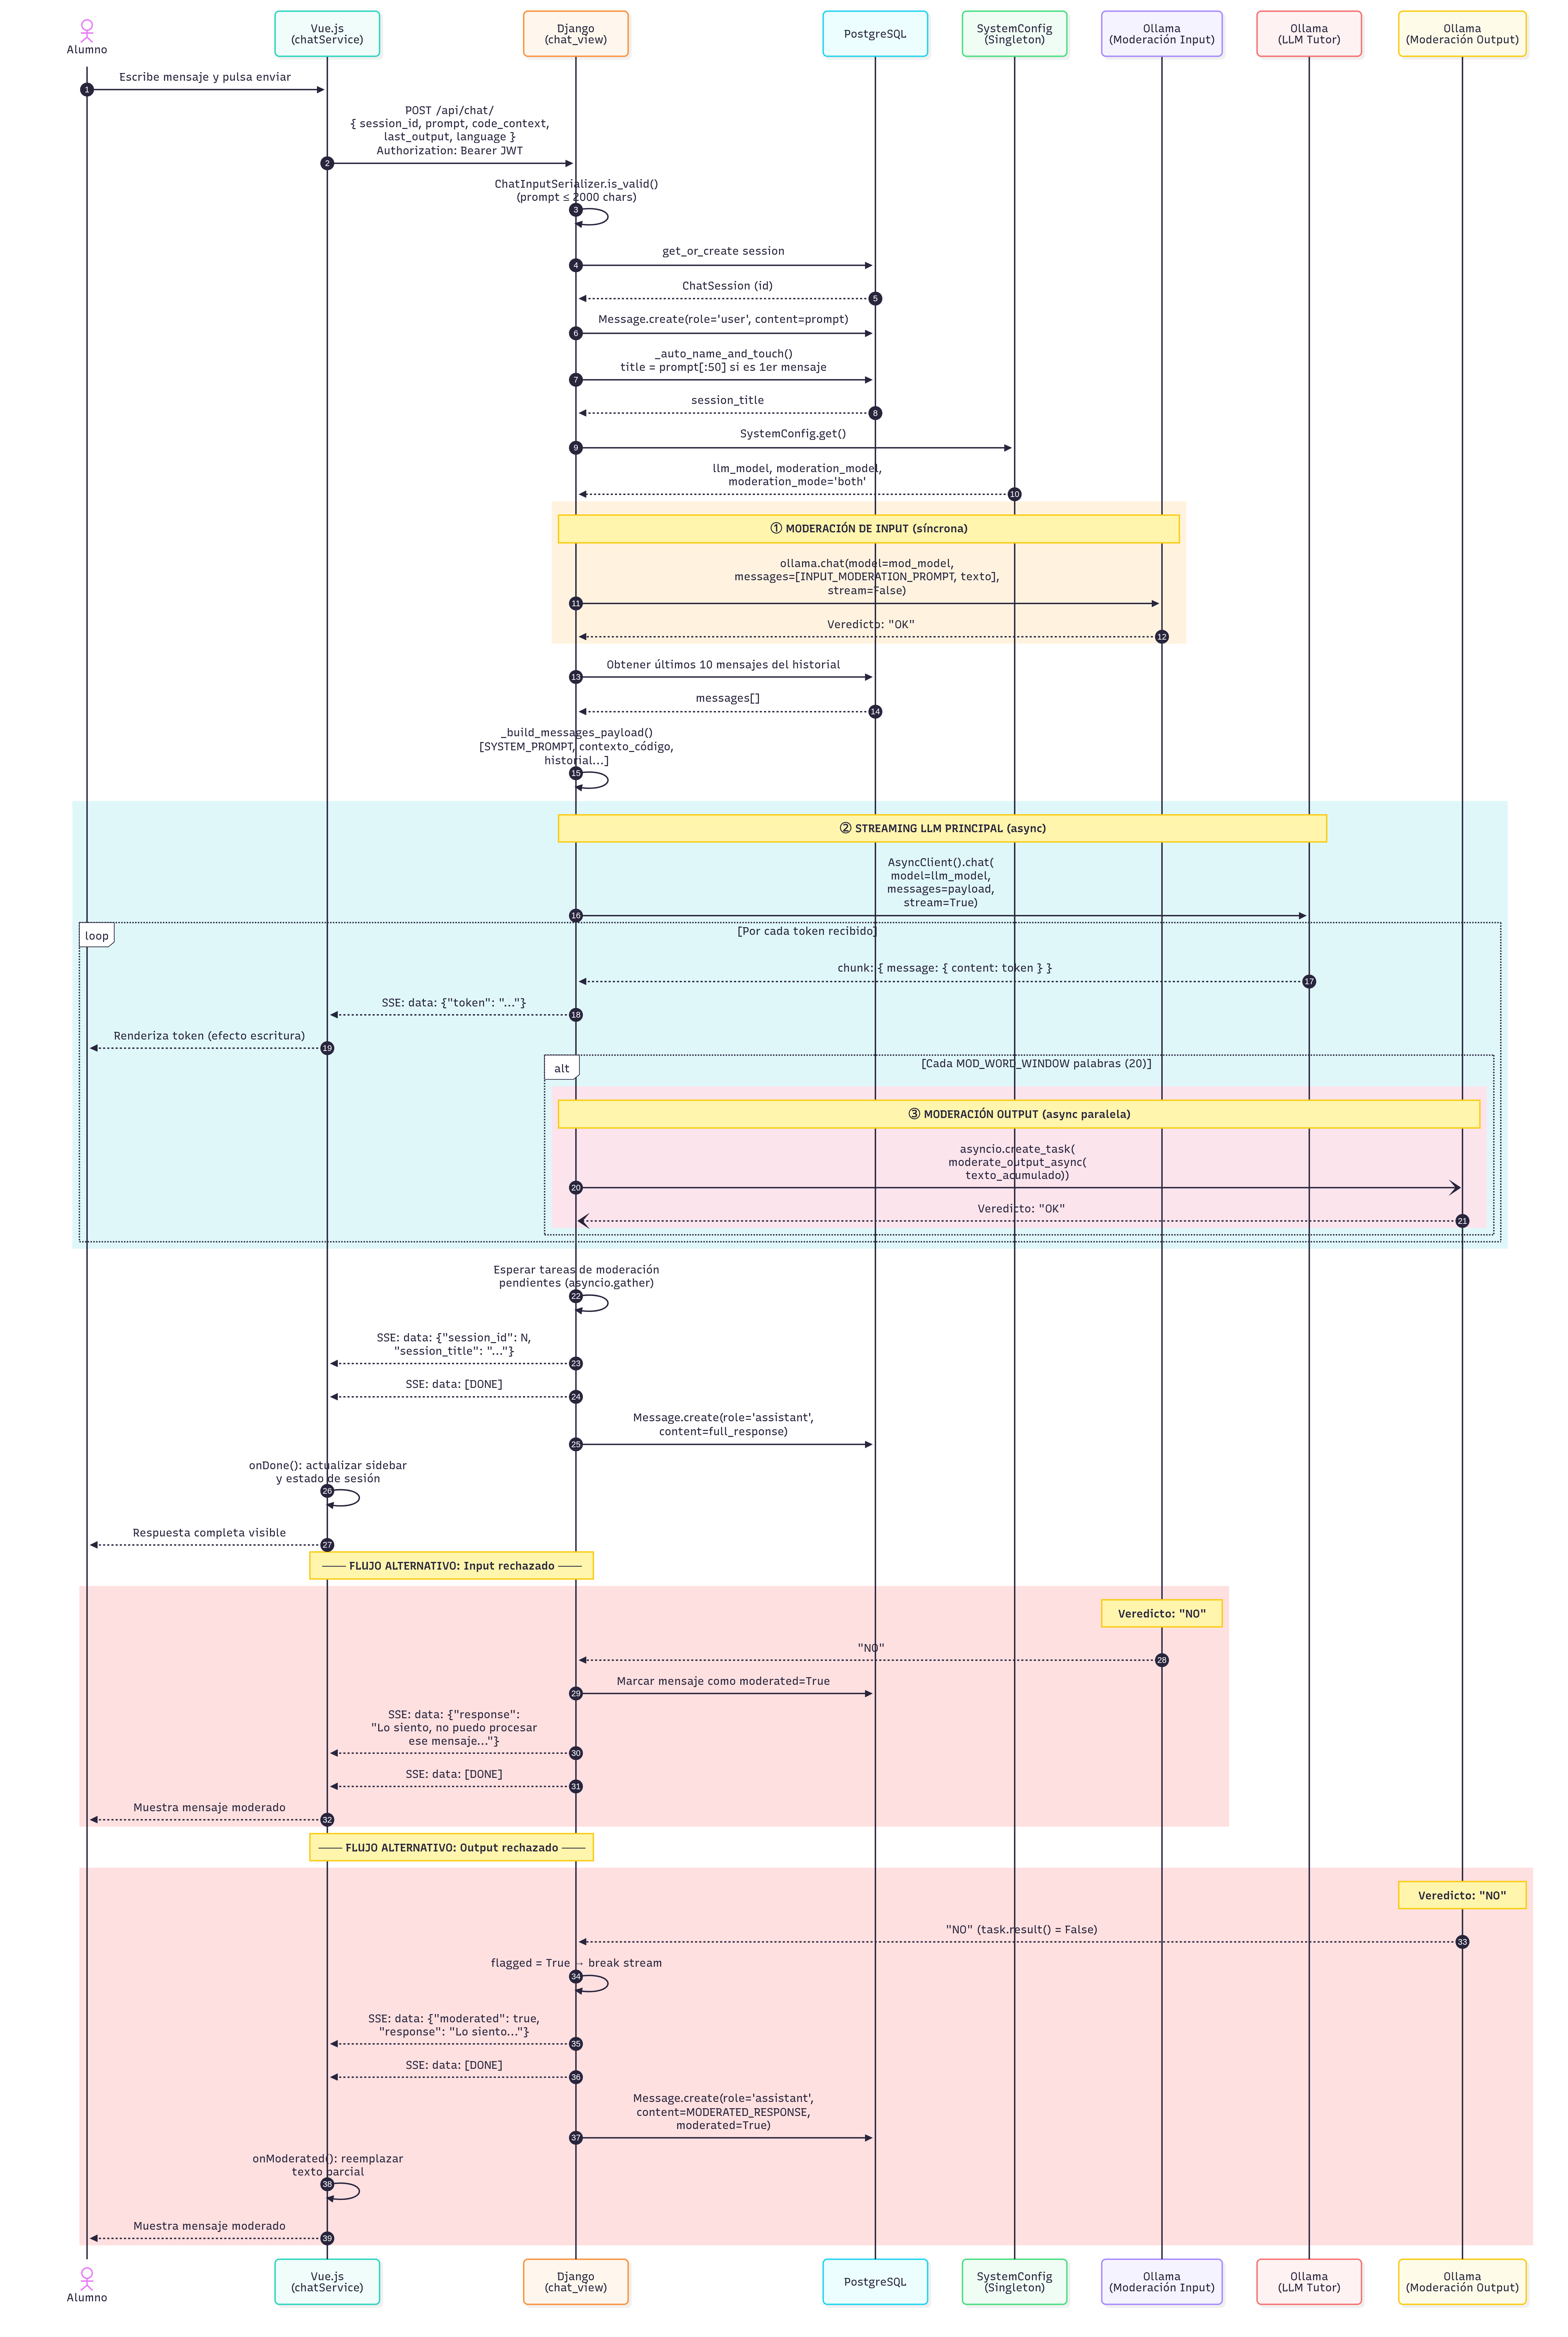
\includegraphics[width=0.85\textwidth]{./diagramas/figura_3-1_secuencia_chat_stream.png}
\end{figure}

\begin{table}[CU2 Ejecución Piston 1]{TB:CU2 1}{Caso de uso: Ejecución de código con Piston. 1}
  \begin{tabular}{l p{11cm}}
    \hline
    \textbf{Campo} & \textbf{Descripción} \\
    \hline \hline
    \textbf{Identificador} & CU2 \\
    \textbf{Nombre} & Compilación y ejecución de código en sandbox \\
    \textbf{Actor principal} & Alumno (usuario autenticado) \\
    \textbf{Actores secundarios} & Piston (contenedor Docker de ejecución de código) \\
    \textbf{Descripción} & El alumno ejecuta el código de su editor en un entorno sandbox aislado (Piston). El sistema envía el código fuente, el lenguaje y la versión al contenedor, y devuelve la salida estándar (\texttt{stdout}), los errores (\texttt{stderr}) y el código de salida. \\
    \textbf{Precondiciones} & 1. El alumno está autenticado (JWT válido). \newline  2. El contenedor Piston (\texttt{tutor\_compiler}) está activo y accesible en \texttt{PISTON\_URL} (por defecto \texttt{http://localhost:2000}). \newline  3. El runtime del lenguaje solicitado está instalado en Piston. \\
    \textbf{Postcondiciones} & 1. El alumno recibe la salida de ejecución (\texttt{stdout}, \texttt{stderr}, \texttt{exit\_code}). \newline  2. No se persiste ningún dato de ejecución en la base de datos (operación efímera). \newline  3. Los archivos temporales en el contenedor se eliminan automáticamente (tmpfs). \\
    \hline
  \end{tabular}
\end{table}

\begin{table}[CU2 Ejecución Piston 2]{TB:CU2 2}{Caso de uso: Ejecución de código con Piston. 2}
  \begin{tabular}{c c p{8cm}}
    \hline
    \textbf{Paso} & \textbf{Actor} & \textbf{Acción} \\
    \hline \hline
    1 & Alumno & Pulsa el botón ''Ejecutar'' en el editor. El frontend envía \texttt{POST /api/compiler/execute/} con \texttt{\{ source\_code, language, version \}}. \\
    2 & Sistema & Valida los datos de entrada mediante \texttt{ExecuteInputSerializer}. Valores por defecto: \texttt{language='python3'}, \texttt{version='3.10.0'}. \\
    3 & Sistema & Construye el payload para la API de Piston: \texttt{\{ language, version, files: [\{ content: source\_code \}] \}}. \\
    4 & Sistema & Envía \texttt{POST} a \texttt{\{PISTON\_URL\}/api/v2/execute} con el payload JSON. Timeout: 30 segundos. \\
    5 & Piston & Ejecuta el código en un sub-contenedor aislado. Para lenguajes compilados (C, Java), primero compila y luego ejecuta. \\
    6 & Piston & Devuelve la respuesta JSON con los campos \texttt{compile} (opcional), \texttt{run.stdout}, \texttt{run.stderr}, \texttt{run.code} y \texttt{run.signal}. \\
    7 & Sistema & Procesa la respuesta: extrae \texttt{stdout}, concatena \texttt{stderr} de compilación y ejecución, extrae \texttt{exit\_code} (o asigna \texttt{-1} si es \texttt{null}). \\
    8 & Sistema & Devuelve al frontend: \texttt{\{ stdout, stderr, exit\_code, language \}} con HTTP 200. \\
    9 & Frontend & Muestra \texttt{stdout} en el panel de salida del editor. Si \texttt{stderr} no está vacío, lo muestra como error. \\
    \hline
  \end{tabular}
\end{table}

\begin{table}[CU2 Ejecución Piston 3]{TB:CU2 3}{Caso de uso: Ejecución de código con Piston. 3}
  \begin{tabular}{c p{8cm} p{8cm}}
    \hline
    \textbf{ID} & \textbf{Condición} & \textbf{Acción del sistema} \\
    \hline \hline
    FA-01 & Piston no accesible (\texttt{ConnectionError}) & Se devuelve HTTP 503 con \texttt{\{''error'': ''No se pudo conectar con el servicio de ejecución de código.'', ''details'': null\}}. \\
    FA-02 & Timeout de ejecución (\texttt{requests.Timeout}) & Se devuelve HTTP 504 con \texttt{\{''error'': ''El servicio de ejecución de código tardó demasiado.'', ''details'': null\}}. \\
    FA-03 & Señal SIGKILL recibida & El programa del alumno ha excedido el límite de tiempo de Piston. Se añade al \texttt{stderr}: \texttt{''[Error del Sistema]: El programa ha superado el límite de tiempo y ha sido detenido. Revisa si tienes un bucle infinito (while True).''} \\
    FA-04 & Error de Piston (campo \texttt{message} en respuesta) & Se devuelve HTTP 400 con el mensaje de error de Piston (ej: lenguaje no instalado). \\
    FA-05 & Error inesperado del servidor & Se devuelve HTTP 500 con \texttt{\{''error'': ''Error inesperado: <detalle>'', ''details'': null\}}. \\
    FA-06 & Error de compilación (lenguajes compilados) & \texttt{compile.stderr} contiene los errores del compilador. Se concatena con \texttt{run.stderr} y se devuelve al alumno como \texttt{stderr}. \\
    \hline
  \end{tabular}
\end{table}

\begin{figure}[Diagrama de secuencia CU2]{FIG:CU2_SEQ}{Diagrama de secuencia de ejecución de código en Piston.}
    \centering
    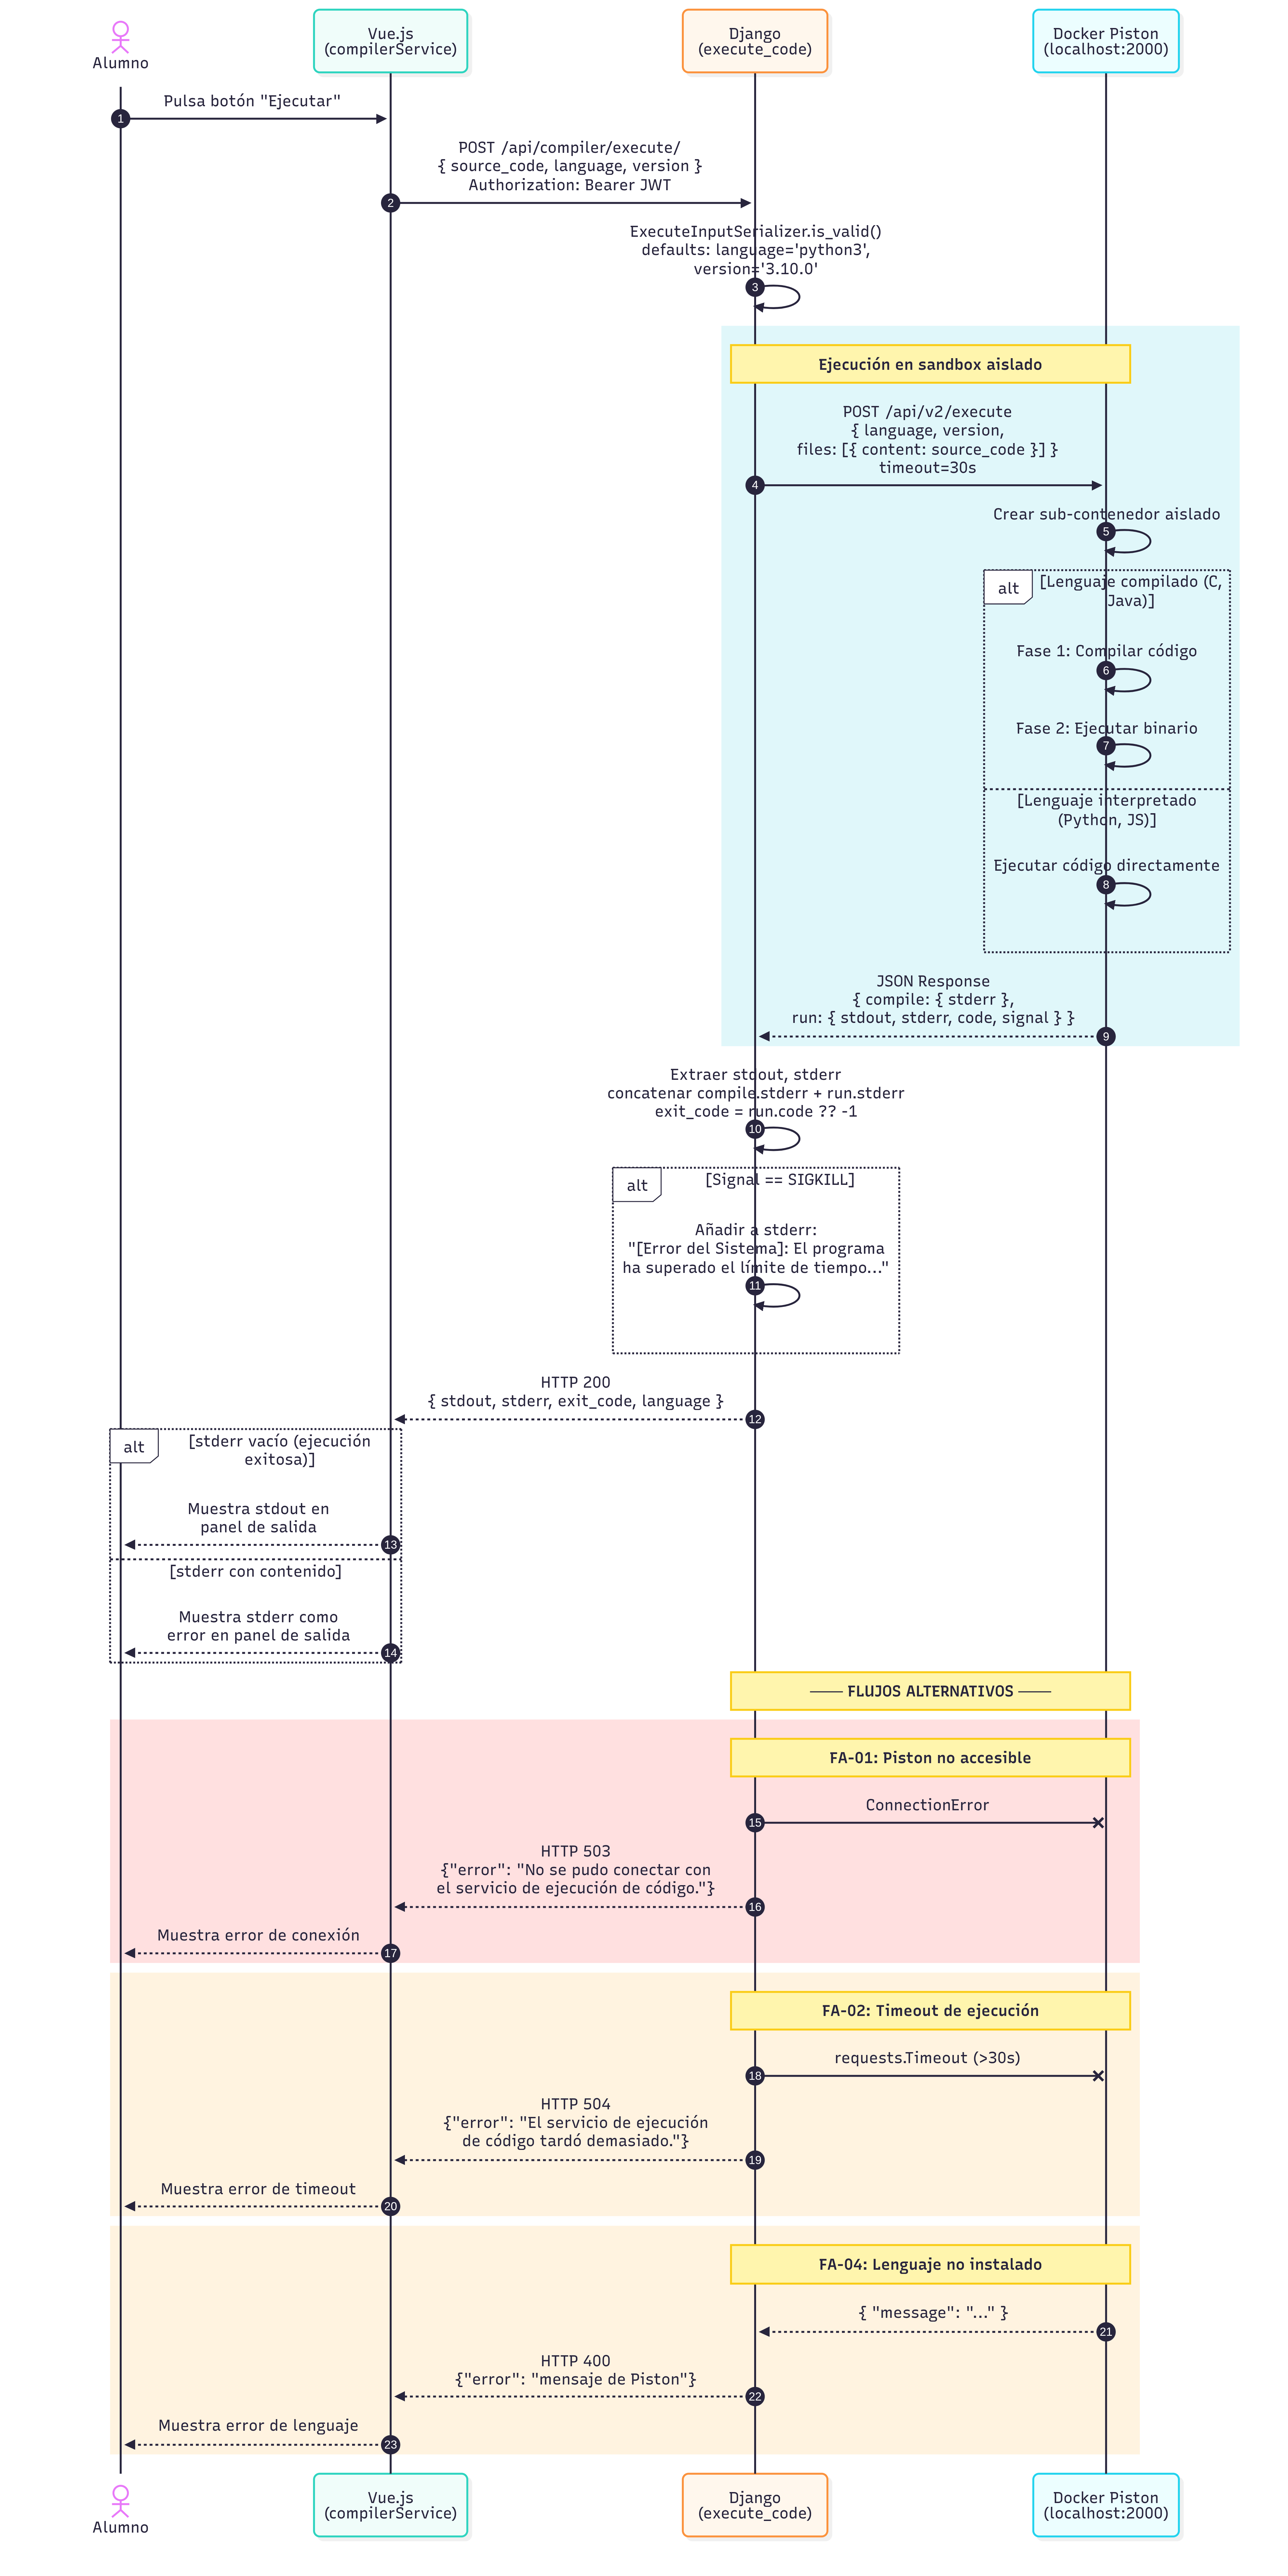
\includegraphics[width=0.85\textwidth]{./diagramas/figura_3-2_secuencia_ejecucion_piston.png}
\end{figure}

\begin{table}[CU3 Configuración Singleton 1]{TB:CU3 1}{Caso de uso: Configuración global del sistema. 1}
  \begin{tabular}{l p{11cm}}
    \hline
    \textbf{Campo} & \textbf{Descripción} \\
    \hline \hline
    \textbf{Identificador} & CU3 \\
    \textbf{Nombre} & Configuración global del sistema (patrón Singleton) \\
    \textbf{Actor principal} & Administrador (usuario con \texttt{is\_staff=True}) \\
    \textbf{Actores secundarios} & — \\
    \textbf{Descripción} & El administrador accede al panel de Django Admin para configurar los parámetros globales del sistema: modelo LLM del tutor, modelo LLM de moderación y modo de moderación. La configuración se almacena en una única fila de la tabla \texttt{SystemConfig} (patrón Singleton). \\
    \textbf{Precondiciones} & 1. El administrador tiene acceso al panel de Django Admin (\texttt{/admin/}). \newline  2. El usuario tiene permisos de staff (\texttt{is\_staff=True}). \\
    \textbf{Postcondiciones} & 1. La configuración queda persistida en la fila con \texttt{pk=1} de \texttt{SystemConfig}. \newline  2. Las peticiones de chat subsiguientes utilizarán los nuevos valores de forma inmediata (lectura en cada petición mediante \texttt{SystemConfig.get()}). \\
    \hline
  \end{tabular}
\end{table}

\begin{table}[CU3 Configuración Singleton 2]{TB:CU3 2}{Caso de uso: Configuración global del sistema. 2}
  \begin{tabular}{c c p{8cm}}
    \hline
    \textbf{Paso} & \textbf{Actor} & \textbf{Acción} \\
    \hline \hline
    1 & Administrador & Accede a \texttt{http://localhost:8000/admin/} e inicia sesión con credenciales de staff. \\
    2 & Sistema & Muestra el panel de administración con la sección ''Configuración del sistema''. \\
    3 & Administrador & Hace clic en ''Configuración del sistema''. El sistema redirige automáticamente al formulario de edición de la única fila existente (\texttt{changelist\_view} $\rightarrow$ \texttt{redirect(pk/change/)}). \\
    4 & Sistema & Muestra el formulario organizado en dos fieldsets: \newline  — \textbf{Moderación de contenido}: campo \texttt{moderation\_mode} (desplegable: Input + Output, Solo Input, Solo Output, Desactivada). \newline  — \textbf{Modelos LLM (Ollama)}: campos \texttt{llm\_model} y \texttt{moderation\_model} (texto libre, ej: \texttt{llama3.2}, \texttt{phi4-mini-reasoning}). \\
    5 & Administrador & Modifica los valores deseados y pulsa ''Guardar''. \\
    6 & Sistema & El método \texttt{save()} sobrescrito fuerza \texttt{self.pk = 1} antes de guardar, garantizando que solo exista una fila (Singleton). Persiste los cambios en PostgreSQL. \\
    7 & Sistema & Muestra confirmación de guardado exitoso. \\
    \hline
  \end{tabular}
\end{table}

\begin{table}[CU3 Configuración Singleton 3]{TB:CU3 3}{Caso de uso: Configuración global del sistema. 3}
  \begin{tabular}{c p{8cm} p{8cm}}
    \hline
    \textbf{ID} & \textbf{Condición} & \textbf{Acción del sistema} \\
    \hline \hline
    FA-01 & No existe configuración previa & El método de clase \texttt{SystemConfig.get()} (invocado por \texttt{changelist\_view}) ejecuta \texttt{get\_or\_create(pk=1)}, creando la fila con valores por defecto: \texttt{moderation\_mode='both'}, \texttt{llm\_model='llama3.2'}, \texttt{moderation\_model='llama3.2'}. \\
    FA-02 & Intento de crear una segunda fila & \texttt{has\_add\_permission()} devuelve \texttt{False} si ya existe una fila, ocultando el botón ''Añadir'' en el Admin. \\
    FA-03 & Intento de eliminar la configuración & \texttt{has\_delete\_permission()} devuelve siempre \texttt{False}, impidiendo el borrado de la configuración. \\
    FA-04 & Modelo LLM no disponible en Ollama & El sistema no valida la existencia del modelo en tiempo de guardado (validación diferida). El error se producirá en la siguiente petición de chat, donde \texttt{ollama.chat()} lanzará una excepción capturada por el flujo de error del CU1 (FA-05). \\
    FA-05 & Acceso por usuario sin permisos de staff & Django Admin deniega el acceso y redirige a la página de login del Admin. \\
    \hline
  \end{tabular}
\end{table}

\begin{table}[CU3 Configuración Singleton 4]{TB:CU3 4}{Caso de uso: Configuración global del sistema. 4}
  \begin{tabular}{l p{11cm}}
    \hline
    \textbf{Mecanismo} & \textbf{Implementación} \\
    \hline \hline
    Forzar PK única & \texttt{save()} sobrescrito: \texttt{self.pk = 1} antes de \texttt{super().save()}. \\
    Creación automática & Método de clase \texttt{get()}: \texttt{cls.objects.get\_or\_create(pk=1)}. \\
    Impedir creación manual & \texttt{has\_add\_permission()} $\rightarrow$ \texttt{not SystemConfig.objects.exists()}. \\
    Impedir eliminación & \texttt{has\_delete\_permission()} $\rightarrow$ \texttt{False}. \\
    Redirección automática & \texttt{changelist\_view()} $\rightarrow$ \texttt{redirect(f'\{obj.pk\}/change/')}. \\
    \hline
  \end{tabular}
\end{table}

\begin{figure}[Diagrama de secuencia CU3]{FIG:CU3_SEQ}{Diagrama de secuencia del proceso de Auto-Naming.}
    \centering
    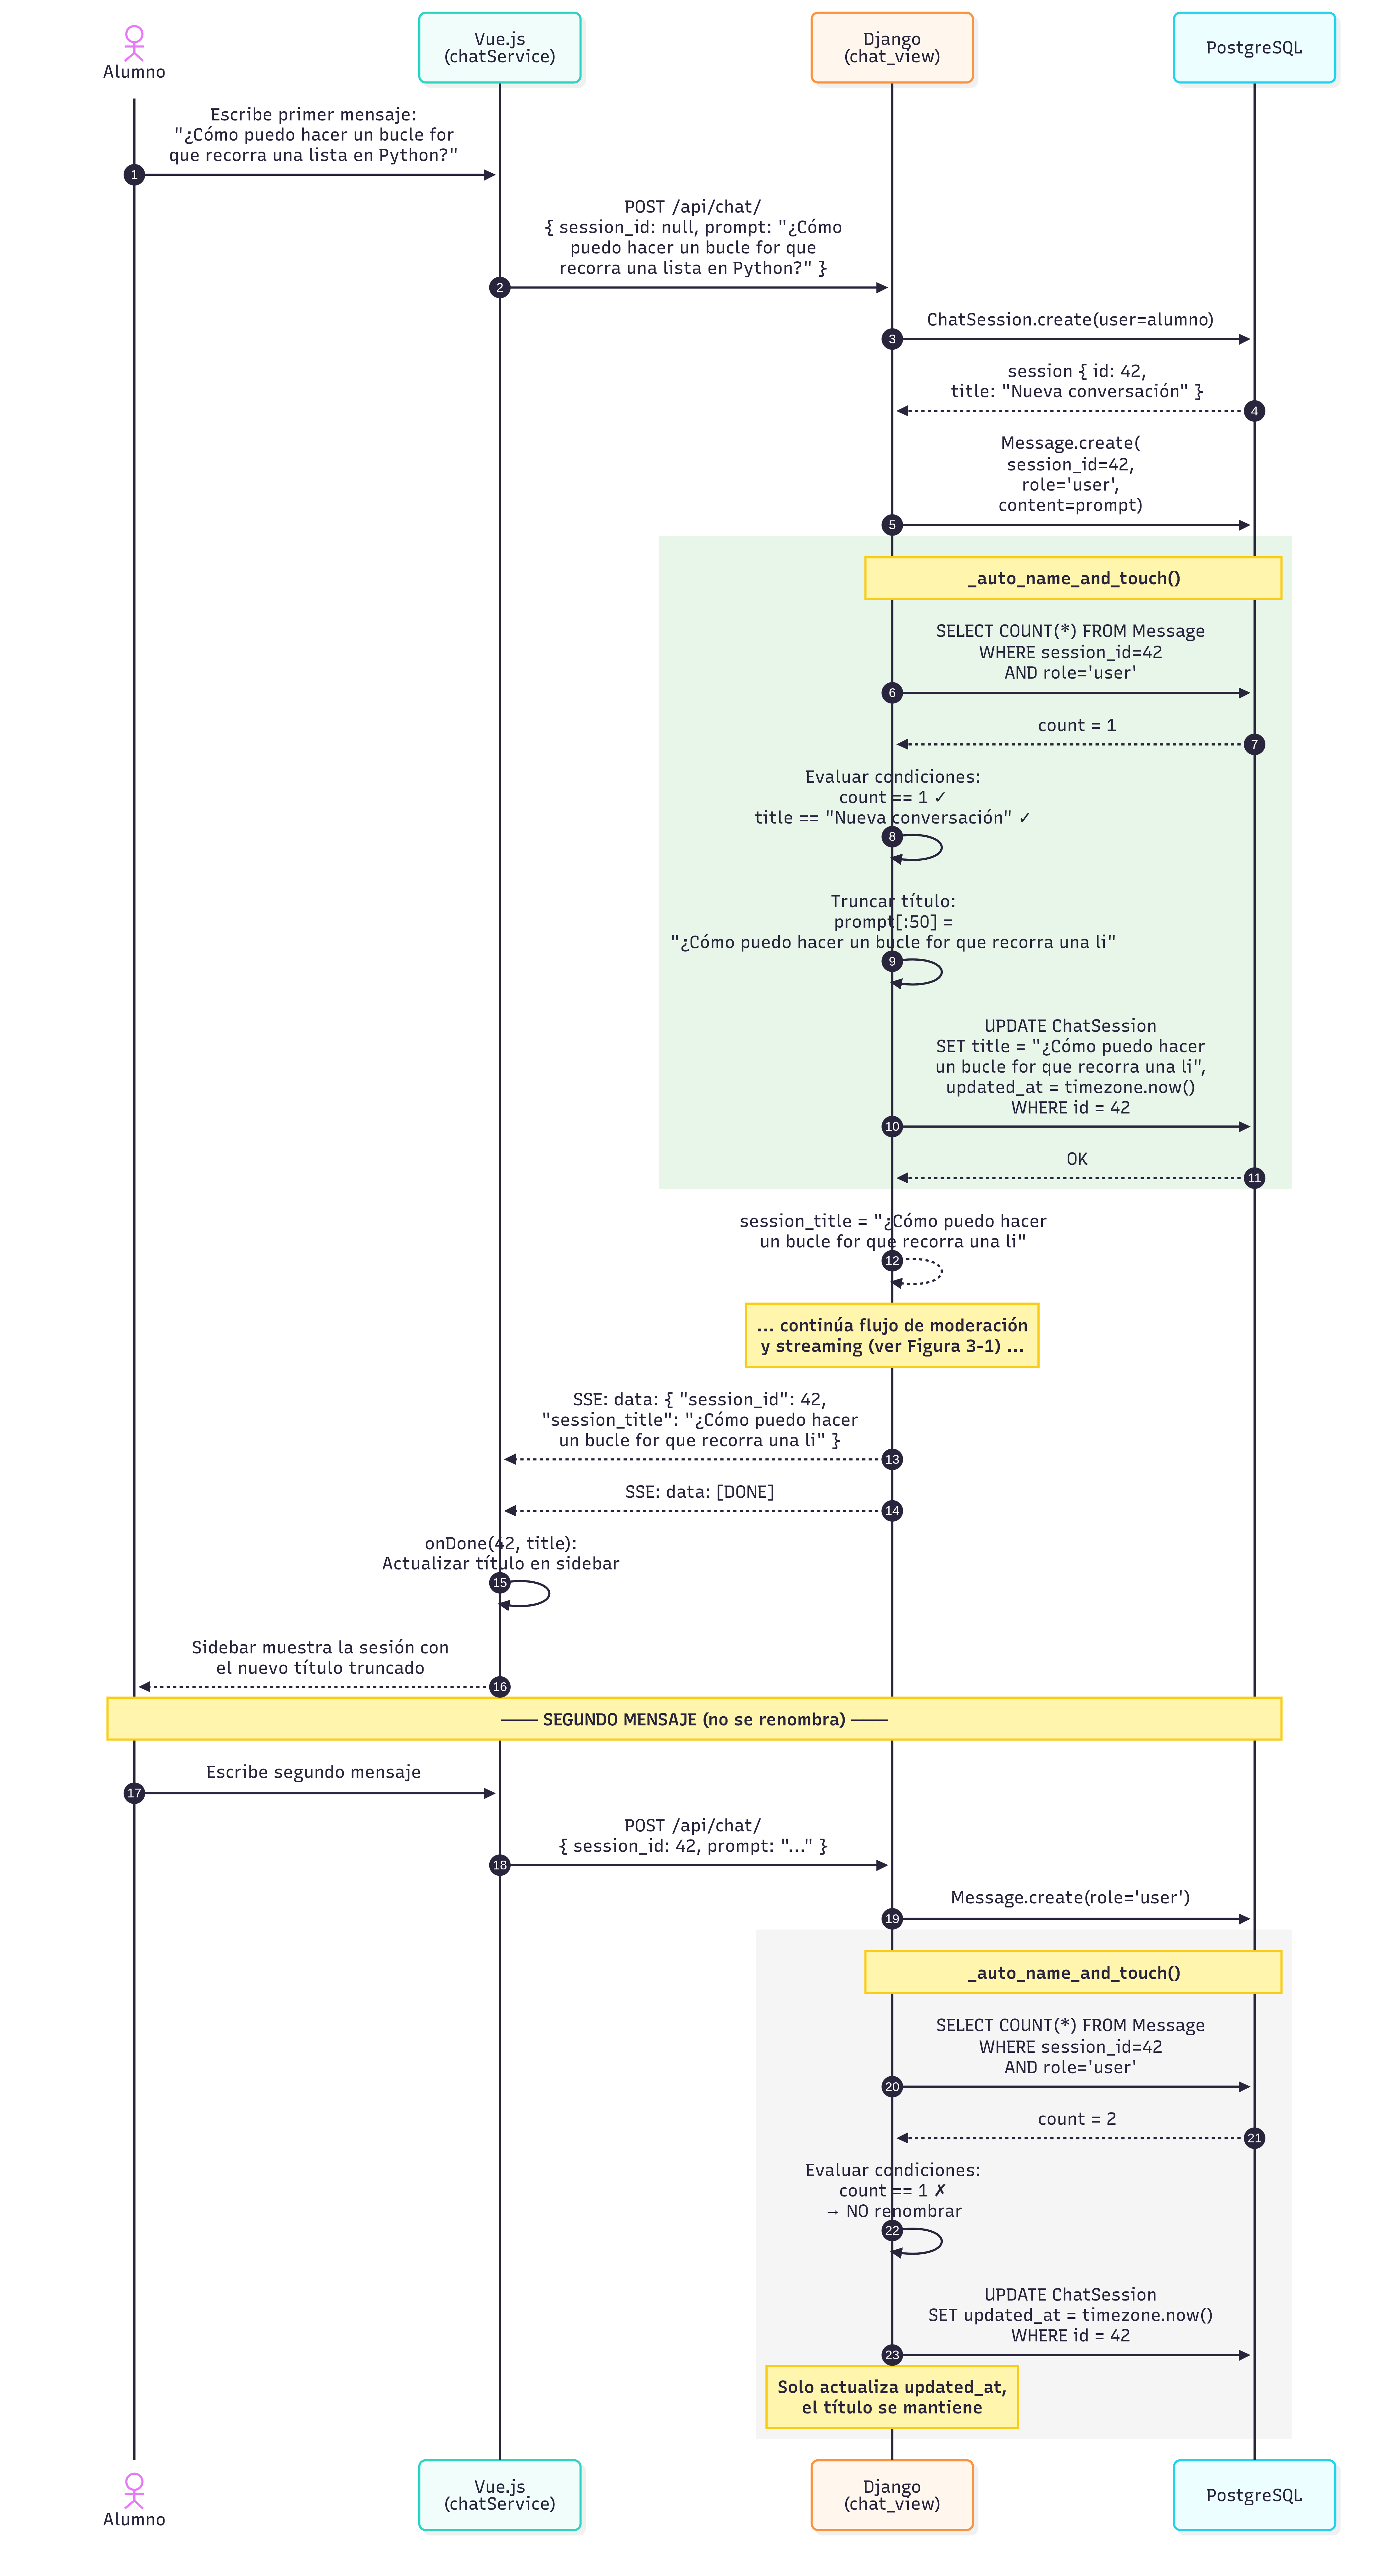
\includegraphics[width=0.85\textwidth]{./diagramas/figura_3-3_secuencia_auto_naming.png}
\end{figure}

